\clearpage
\pagestyle{plain}
\thispagestyle{empty}
\linespread{1.5}
\noindent\huge \color{red}{2017 臺灣維管束植物紅皮書名錄} \\
\noindent\Large \color{red}{The Red List of Vascular Plants of Taiwan, 2017} \\
\normalsize
\hrule
\color{black}
\begin{table}[H]
  \scriptsize
  {\renewcommand\arraystretch{1.2}
  \begin{tabular}{>{\raggedleft\arraybackslash}p{2.5cm}p{9cm}p{3cm}}
      \textbf{引用方式}          & 臺灣植物紅皮書編輯委員會(2017) 
                                        2017 臺灣維管束植物紅皮書名錄。
                                        行政院農業委員會特有生物研究保育中心、行政院農業委員會林務局、臺灣植物分類學會。南投。 & \\
      \textbf{發行人}                 & 楊嘉棟、林華慶、劉和義  & \\
      \textbf{作者}                   & 臺灣植物紅皮書編輯委員會  & \\
      \textbf{編輯委員會}             & 2008--2010: 王震哲(召集人,國立臺灣師範大學)、邱文良(林業試驗所)、
                                        張和明(特有生物研究保育中心)、許再文(特有生物研究保育中心)、
                                        郭長生(國立成功大學)、彭鏡毅(中央研究院)、楊國禎 (靜宜大學)、
                                        劉和義(國立中山大學)、謝長富(國立臺灣大學)  & \\
                                      & 2017: 王志強(國立屏東科技大學)、江友中(國立中山大學)、林政道(國立嘉義大學)、
                                        張和明(特有生物研究保育中心)、許再文(特有生物研究保育中心)、
                                        曾彥學(國立中興大學)、劉以誠(國立嘉義大學)、劉和義(召集人,國立中山大學)、
                                        謝宗欣(國立臺南大學)、鍾國芳(中央研究院)  & \\
      \textbf{執行編輯}          & 張和明、劉和義、許再文、林政道  & \\
      \textbf{助理編輯}          & 楊松翰、劉瓊芳、廖國藩  & \\
      \textbf{出版}              & 行政院農業委員會特有生物研究保育中心、行政院農業委員會林務局、臺灣植物分類學會  & \\
      \textbf{地址}              & 55244 臺灣南投縣集集鎮民生東路 1 號  & \\
      \textbf{出版年月}          & 2017 年 12 月  & \\
      \textbf{ISBN}              & 978-986-05-5021-4  & \\
      \textbf{GPN}               & 1010602773  & \\
      \textbf{資料下載}          & \href{http://tesri.tesri.gov.tw}{特有生物研究保育中心 網址:http://tesri.tesri.gov.tw}  & \\
                                 & \href{http://www.tsps.org.tw}{臺灣植物分類學會 網址:http://www.tsps.org.tw}  & \\
      \textbf{定價}              & 新臺幣 350 元  & \\
      \textbf{授權}              & 本報告依據
                                   \href{https://creativecommons.org/licenses/by/4.0}{Creative Commons Attribution 4.0 International License}
                                   授權,使用者可進行重製散布、重混、調整,以及依原著作建立新著作(包括商業與非商業性利用),
                                   惟使用時必須引用按照指定方式註明來源。  & \\
      \textbf{版本}              & 20180309 \\
      \textbf{Citation}          & Editorial Committee of the Red List of Taiwan Plants (2017) The Red List of Vascular Plants of Taiwan, 2017.
                                   Endemic Species Research Institute, Forestry Bureau, Council of Agriculture, 
                                   Executive Yuan and Taiwan Society of Plant Systematics.  & \\
      \textbf{Publisher}         & Yang, Jia-Dong; Lin, Hwa-Ching Lin; Liu, Ho-Yih  & \multirow{13}{*}{
      \shortstack[l]{
      封底照片 \\
      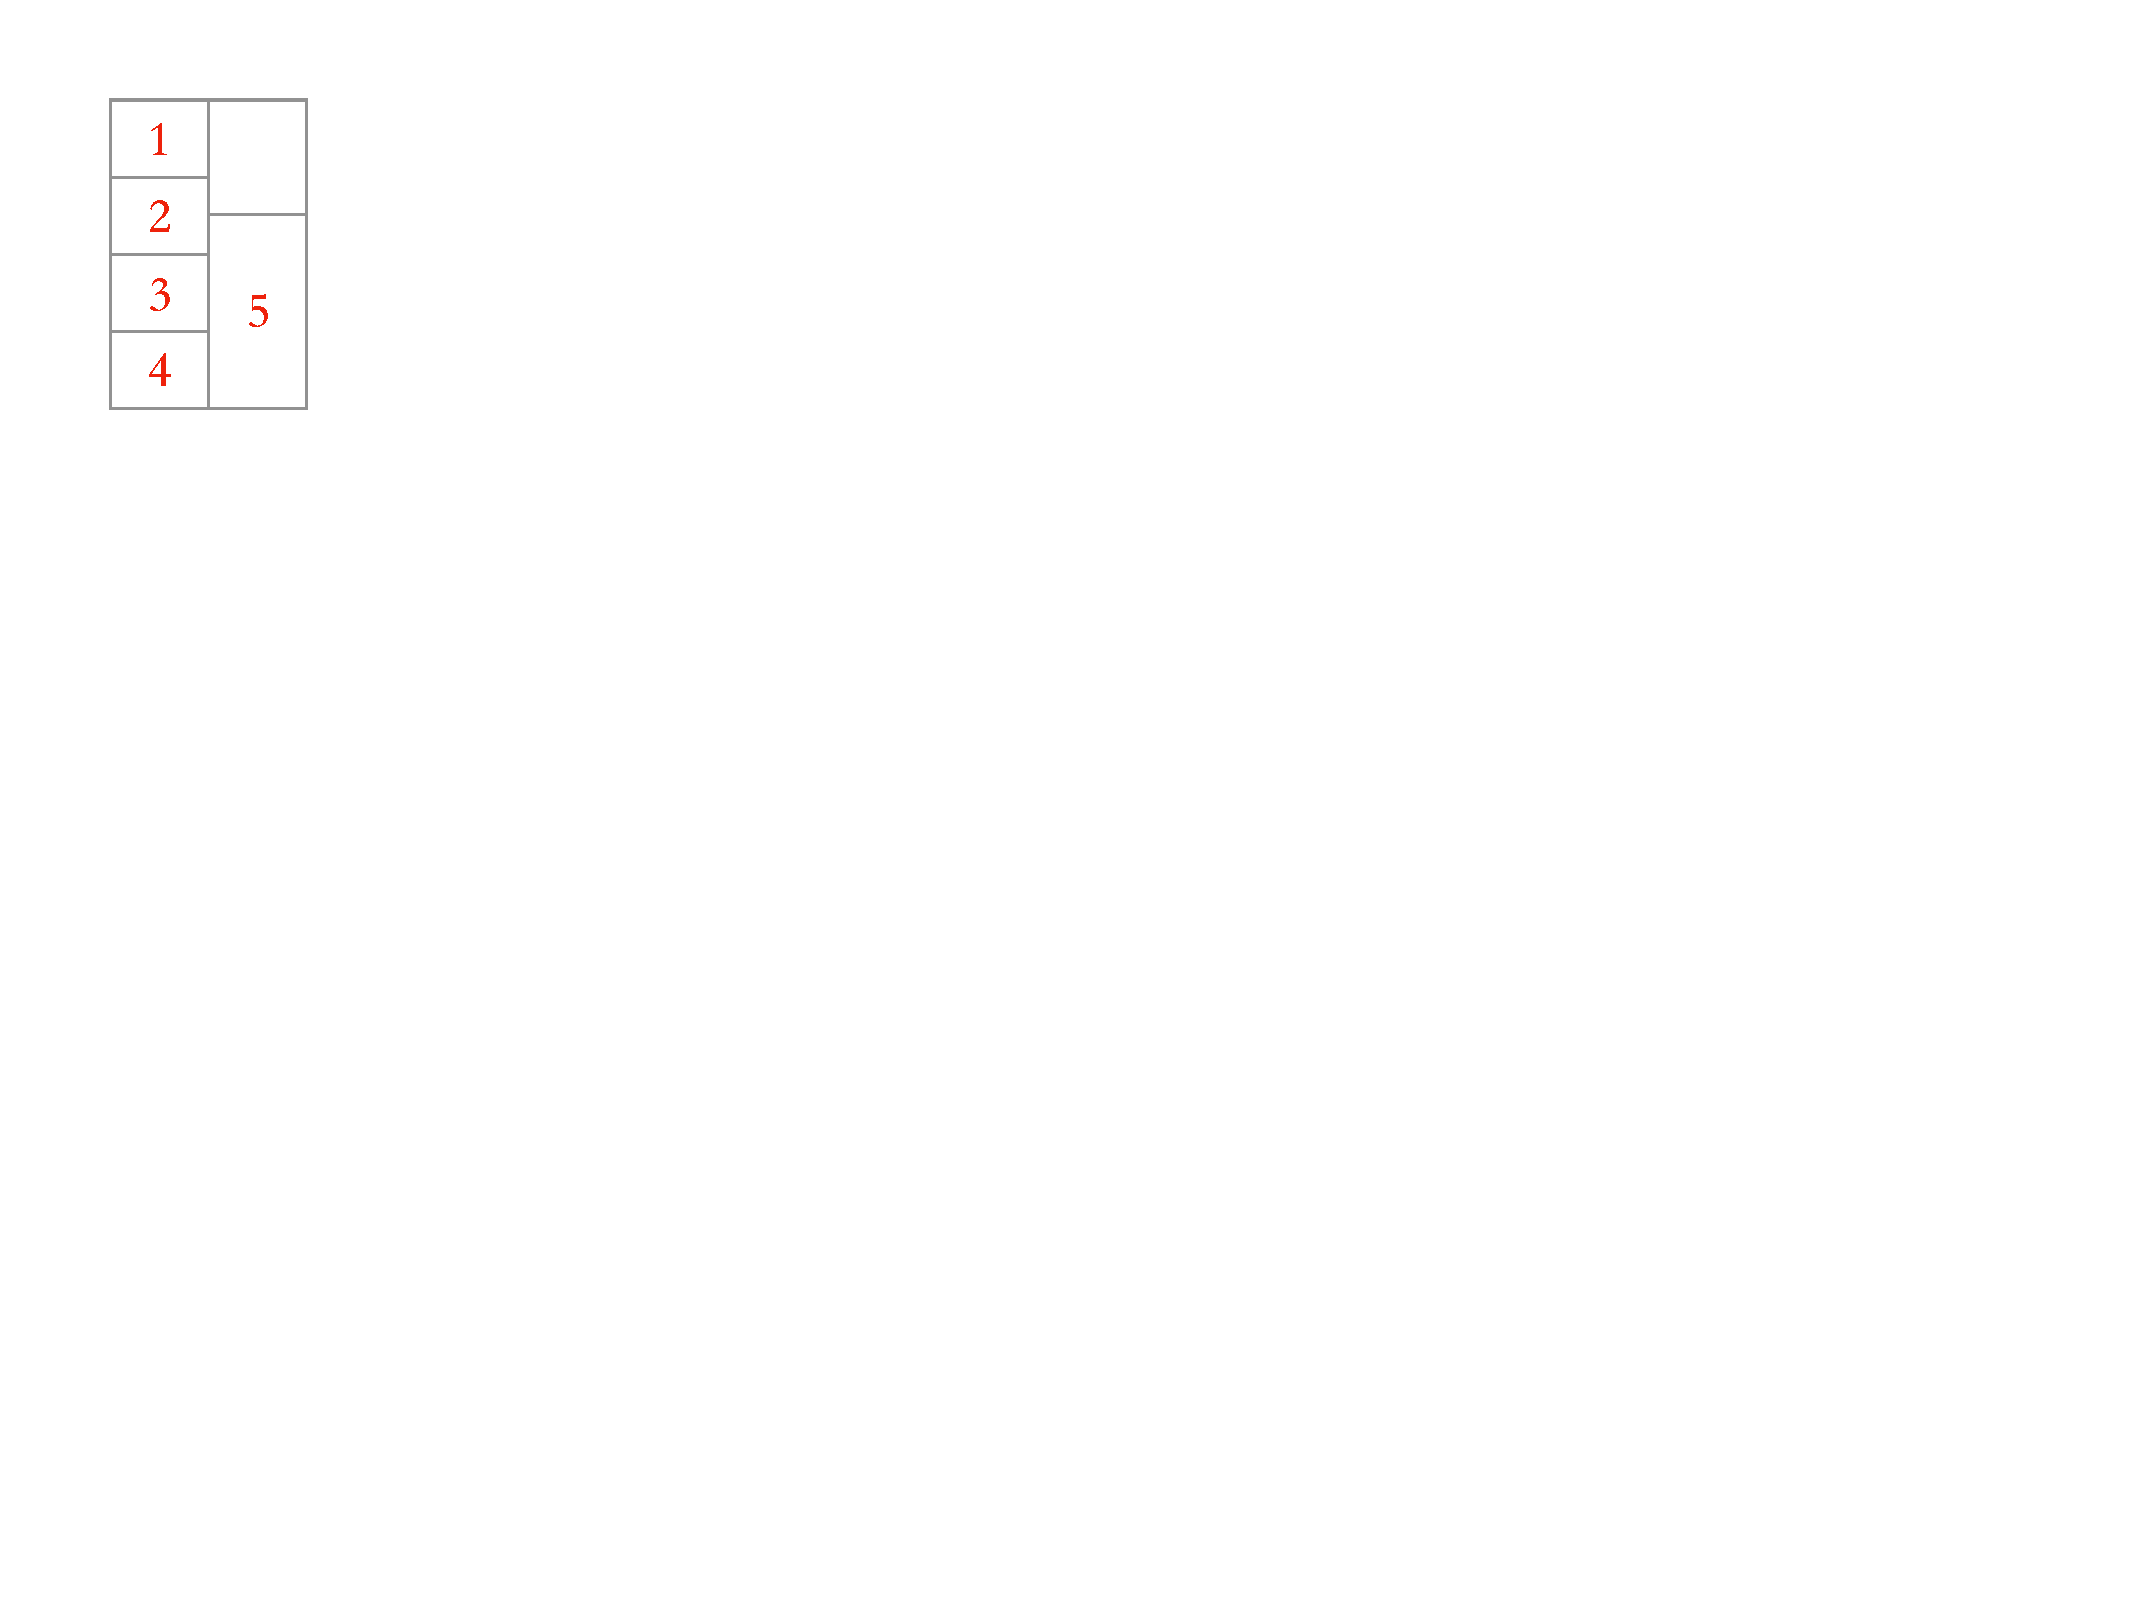
\includegraphics[width=2.5cm]{images/coverback.pdf} \\
      \textcolor{red}{\bfseries{1}} {\mbox{\color{red}\rule[-0.5mm]{1mm}{0.34cm}~~}}
        \textit{Dryopteris dickinsii} (Franchet \& Savatier) \\ 
        ~~~~~~~~~~C.Christense \\ 
        ~~~~~~~遠軸鱗毛蕨~~EN* D \\
        ~~~~~~~呂碧鳳/攝 \\
      \textcolor{red}{\bfseries{2}} {\mbox{\color{red}\rule[-0.5mm]{1mm}{0.34cm}~~}}
        \textit{Lilium speciosum} Thunb. var. \textit{oriosoides} \\ 
        ~~~~~~~豔紅鹿子百合~~CR C1\\
        ~~~~~~~蔡依恆/攝\\
      \textcolor{red}{\bfseries{3}} {\mbox{\color{red}\rule[-0.5mm]{1mm}{0.34cm}~~}}
        \textit{Argyreia akoensis} S.Z.Yang, P.H.Chen \& \\
        ~~~~~~~~~~G.W.Staples \\
        ~~~~~~~屏東朝顏~~CR B1a+2a; D1; D2\\
        ~~~~~~~楊勝任/攝\\
      \textcolor{red}{\bfseries{4}} {\mbox{\color{red}\rule[-0.5mm]{1mm}{0.34cm}~~}}
        \textit{Trapa japonica} Flerow \\ 
        ~~~~~~~日本菱~~CR B1ab(iii)+2ab(iii)\\
        ~~~~~~~黃朝慶/攝\\
      \textcolor{red}{\bfseries{5}} {\mbox{\color{red}\rule[-0.5mm]{1mm}{0.34cm}~~}}
        \textit{Appendicula lucbanensis} (Ames) Ames \\ 
        ~~~~~~~多枝竹節蘭~~CR B2ab(iii)\\
        ~~~~~~~許天銓/攝~
        }
      } \\ 
      \textbf{Authors}           & Editorial Committee of the Red List of Taiwan Plants  & \\
      \textbf{Editorial Committee} & 2008--2010: Wang, Jenn-Che (coordinator);
                                     Chang, Ho-Ming;
                                     Chiou, Wen-Liang;
                                     Hsieh, Chang-Fu;
                                     Hsu, Tsai-Wen;
                                     Kuo, Chang-Sheng;
                                     Liu, Ho-Yih;
                                     Peng, Ching-I;
                                     Yang, Kuoh-Cheng  & \\
                                   &  2017: Liu, Ho-Yih (coordinator);
                                     Chang, Ho-Ming;
                                     Chiang, Yu-Chung;
                                     Chung, Kuo-Fang;
                                     Hsieh, Tsung-Hsin; 
                                     Lin, Cheng-Tao;
                                     Liu, Yea-Chen;
                                     Tzeng, Yen-Hsueh; 
                                     Wang, Chih-Chiang  & \\
      \textbf{Executive Editors}  & Chang, Ho-Ming; Liu, Ho-Yih; Hsu, Tsai-Wen; Lin, Cheng-Tao  & \\
      \textbf{Associate Editors}  & Yang, Song-Han; Liu, Chun-Fang; Liao, Guo-Fang  & \\
      \textbf{Published by}       & Endemic Species Research Institute, COA, EY, Taiwan.
                                    Forestry Bureau, Council of Agriculture, COA, EY, Taiwan.
                                    Taiwan Society of Plant Systematics  & \\
      \textbf{Address}            & No. 1, Ming-Shen East Road, Jiji Township, Nantou County, 55244, Taiwan  & \\
      \textbf{Published Date}     & December 2017  & \\
      \textbf{ISBN}               & 978-986-05-5021-4  & \\
      \textbf{GPN}                & 1010602773  & \\
      \textbf{Download URL}  & \href{http://tesri.tesri.gov.tw}{Taiwan Endemic Species Research Institute URL:http://tesri.tesri.gov.tw}  & \\
                                  & \href{http://www.tsps.org.tw}{Taiwan Society of Plant Systematics URL: http://www.tsps.org.tw}  & \\
      \textbf{Price}              & NTD 350  & \\
      \textbf{License}            & \href{https://creativecommons.org/licenses/by/4.0}{Creative Commons Attribution 4.0 International License}.
                                     You must give appropriate credit, provide a link to the license,
                                     and indicate if changes were made. You may do so in any reasonable manner,
                                     but not in any way that suggests the licensor endorses you or your use.  & \\
  \end{tabular}
  }
  \begin{tabular}{p{2.5cm}p{3cm}p{1.0cm}p{1.6cm}p{1.6cm}}
    & 
\includegraphics[width=10em]{images/ccby40.png} & &
    
\includegraphics[width=1.4cm]{images/tesri.png} &
    
\includegraphics[width=1.4cm]{images/tsps.png} \\
  \end{tabular}

\end{table}
%\clearpage
%\thispagestyle{empty}
%\hfill
%\vfill
%{\raggedright\vfill
%   \hfill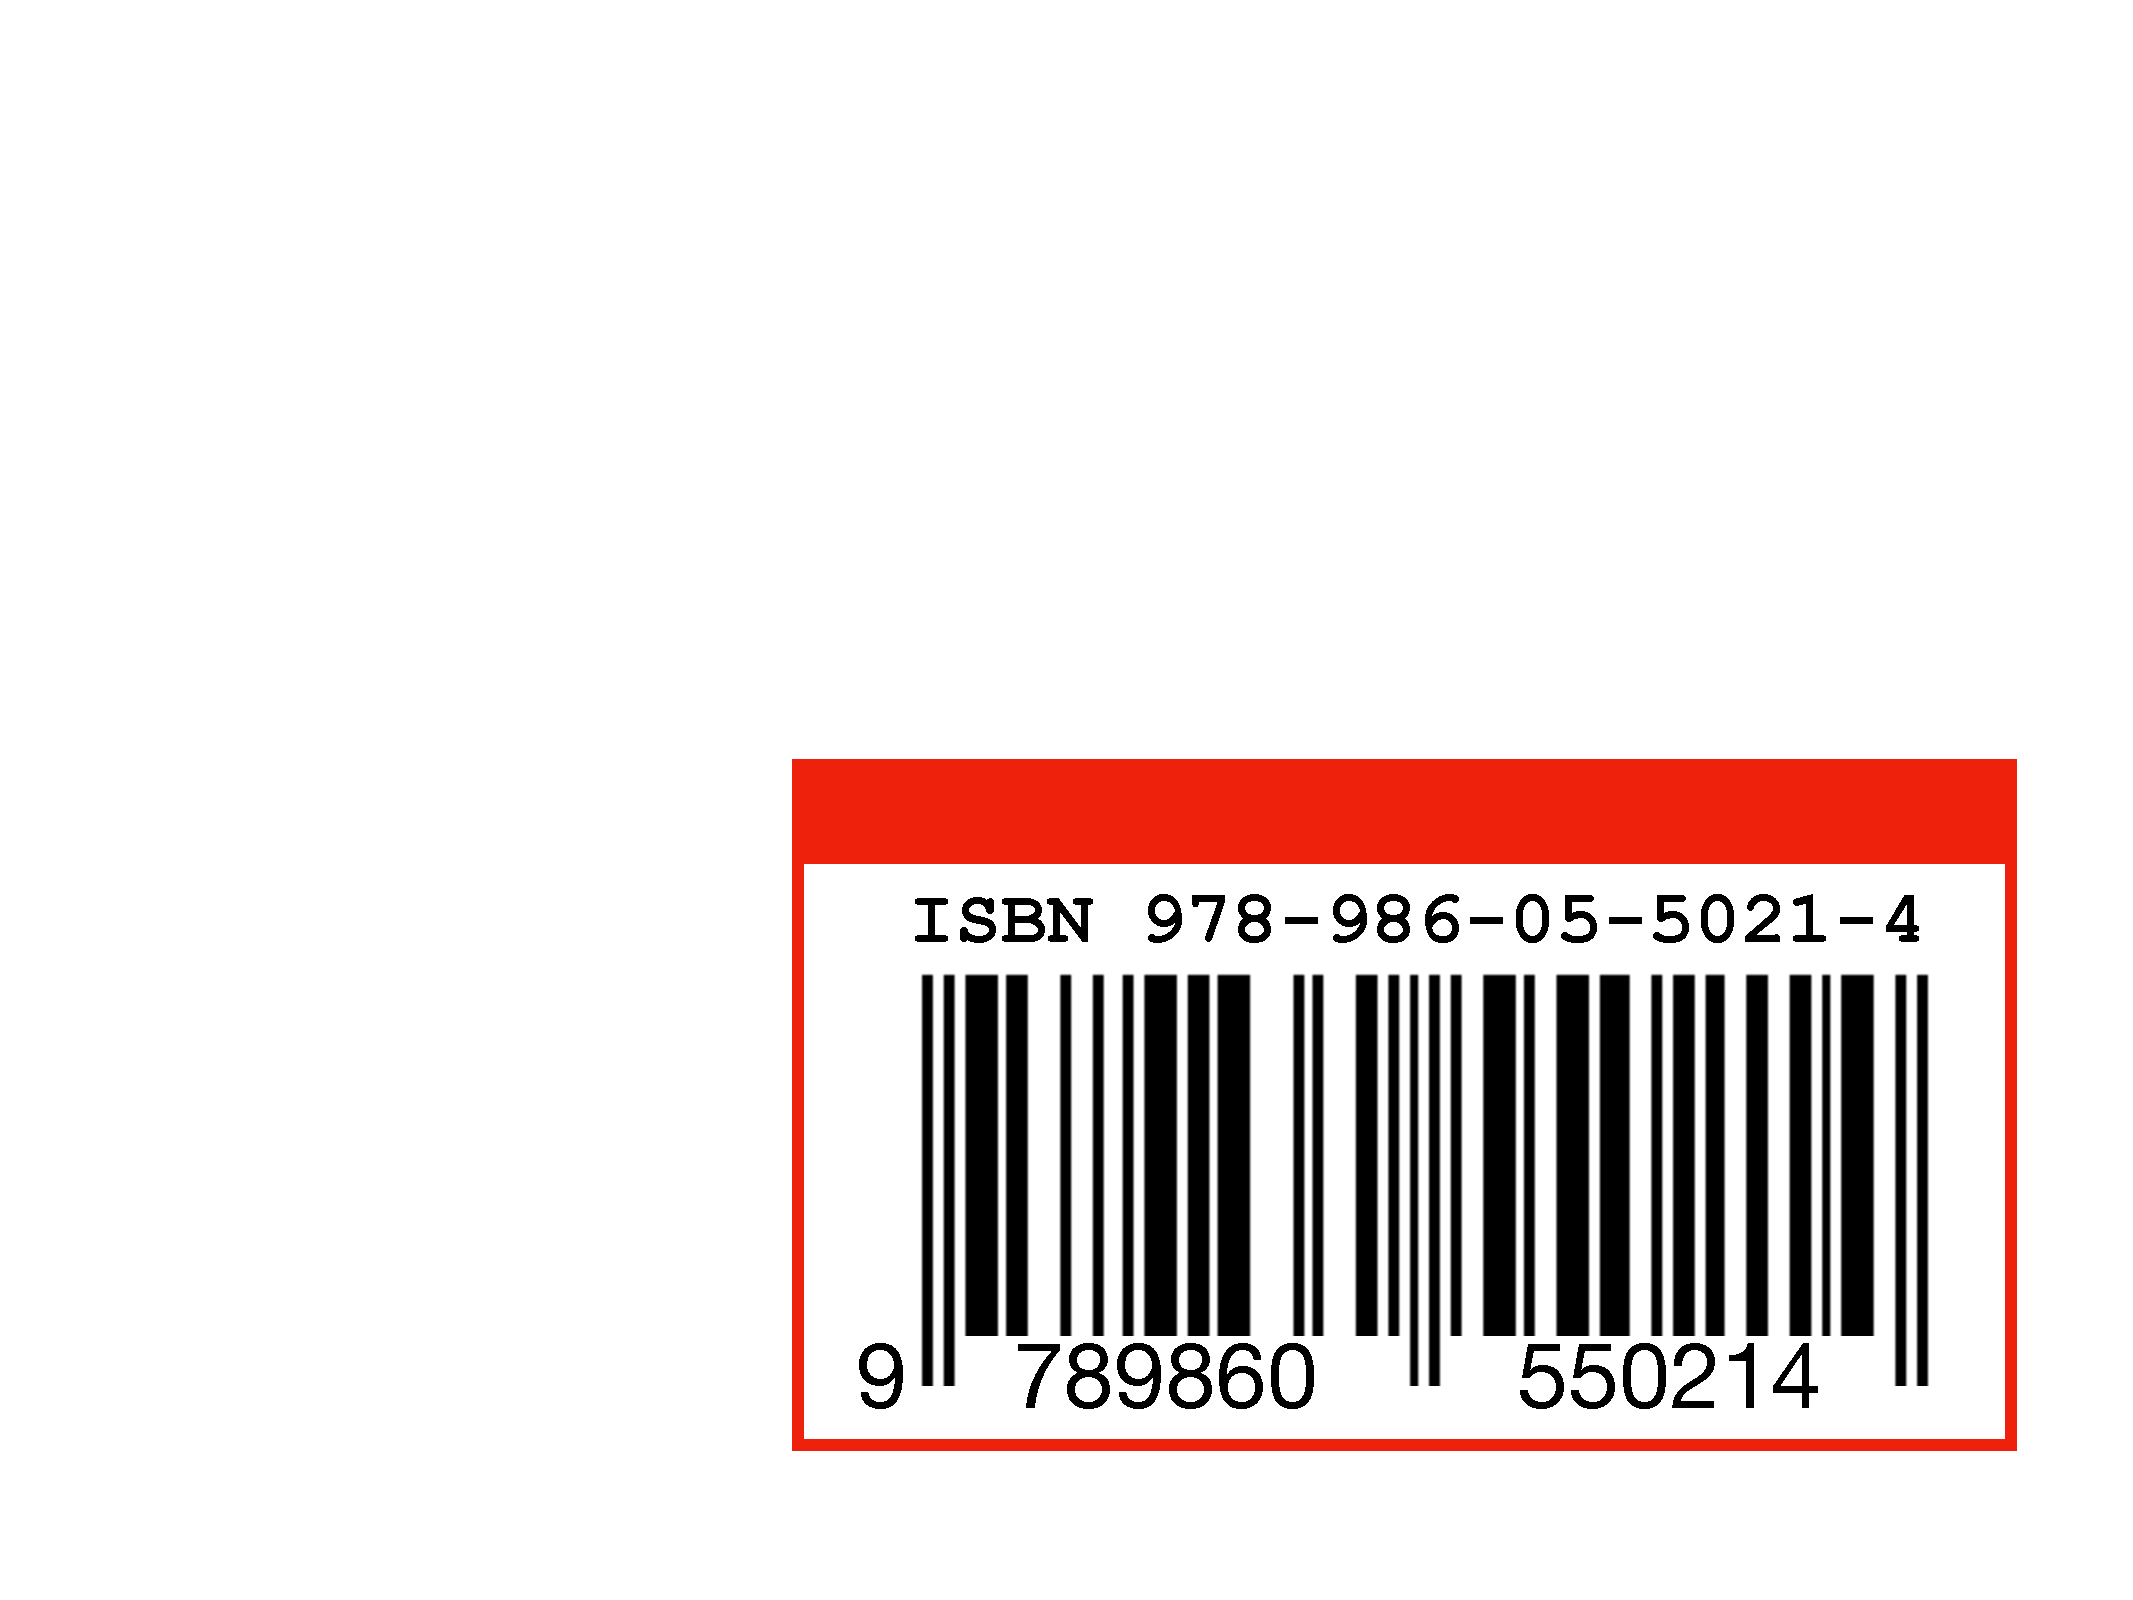
\includegraphics[width=5cm]{images/isbn_final.pdf}
%}
